\chapter[Constructing Voronoi Diagrams Computationally]{Constructing Voronoi Diagrams Computationally}
\label{app:vorchull}

Voronoi diagrams can be efficiently computed using a sweep line algorithm \cite{Fortune1987}.
An excellent library which implements a range of Voronoi methods is Voro\texttt{++} \cite{Rycroft2009}.
However, Voronoi diagrams can also be constructed computationally by utilising an interesting relationship between the Delaunay triangulation of a $D$ dimensional point set and the convex hull of a transformed point set in $D+1$ dimensions.

Given a \td{} point set of particle positions, $\left(x_i,y_i\right)$, one can define the lifting transform, $T : {\rm I\!R}^2\rightarrow {\rm I\!R}^3$, as:
\begin{align}
	T\left(x_i,y_i\right) = \left(x_i,y_i,x_i^2+y_i^2-w_i^2\right),
\end{align}
where $w_i$ are the particle weights.
In the case of the unweighted Voronoi, $T$ corresponds to mapping the points onto a paraboloid.
Now the interesting part is that if the lower convex hull of the transformed points is calculated and projected back onto the original plane, the Delaunay triangulation is obtained \cite{Aurenhammer1987,Okabe1992}.
This holds despite the fact that the Voronoi diagrams are based on the metric properties, whilst convex hulls depend only on affine properties.
Given the Delaunay triangulation, the Voronoi polygons can then be trivially determined.
This process is demonstrated in figures \ref{appfig:vorconvexhull1}--\ref{appfig:vorconvexhull4}.

An advantage of this method is that optimised convex hull algorithms are readily available, whereas modified Voronoi codes are less so.
It is also generalisable to arbitrary dimensions.

\begin{figure}[bt]
	\centering
     
          \begin{subfigure}[b]{0.4\textwidth}
         \centering
         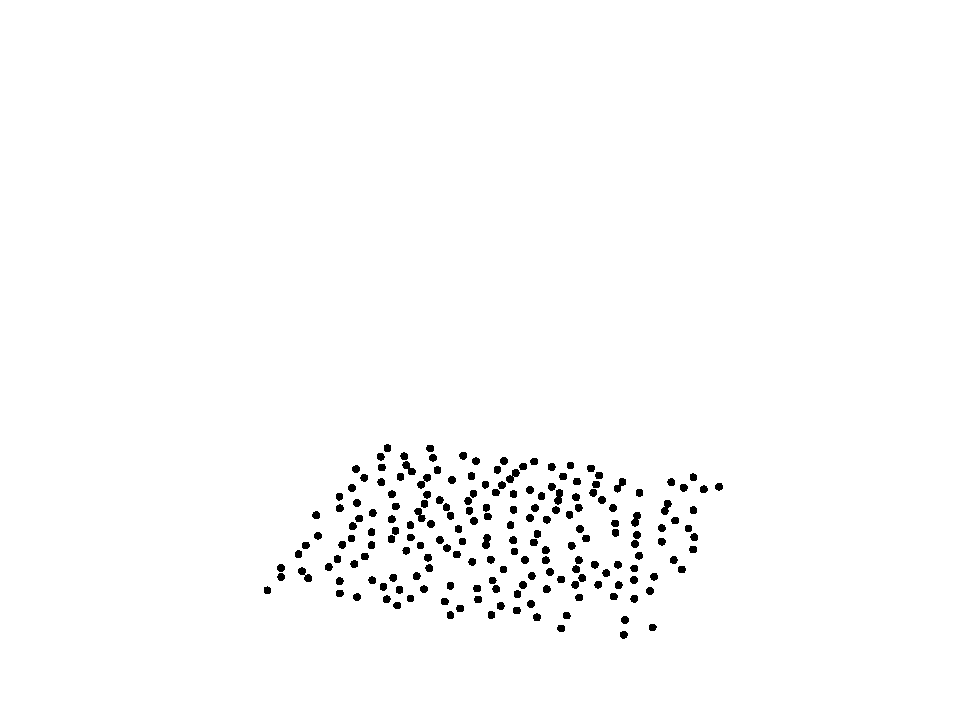
\includegraphics[width=\textwidth]{./appendices/figures/power_1.pdf}
         \caption{}
         \label{appfig:vorconvexhull1}
     \end{subfigure}
   	\hspace{1cm}
      \begin{subfigure}[b]{0.4\textwidth}
         \centering
         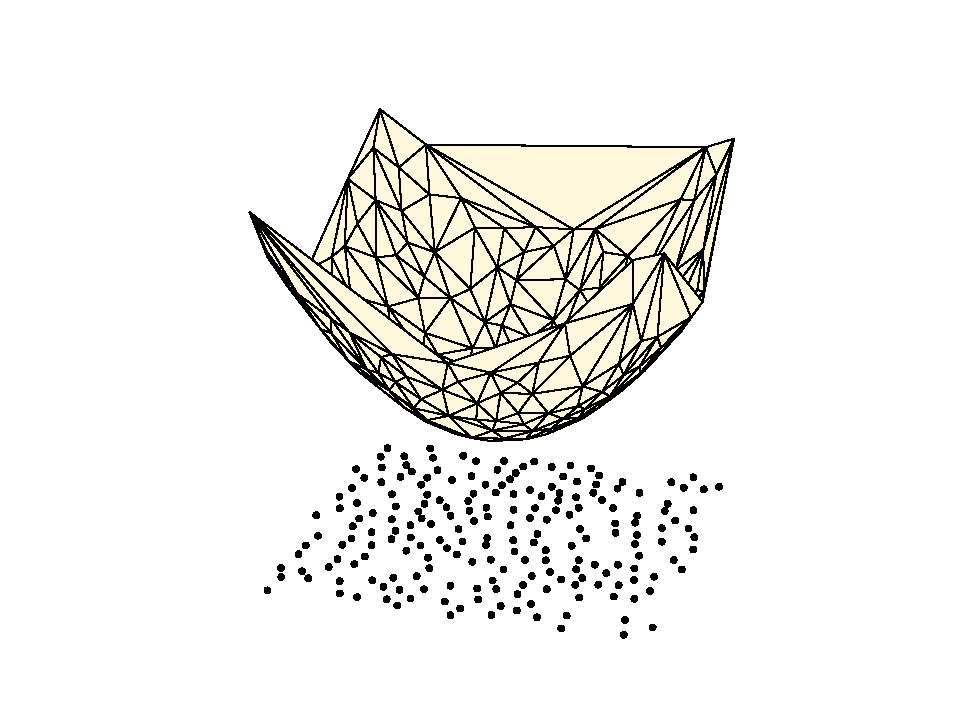
\includegraphics[width=\textwidth]{./appendices/figures/power_2.pdf}
         \caption{}
         \label{appfig:vorconvexhull2}
     \end{subfigure}
     
       \begin{subfigure}[b]{0.4\textwidth}
         \centering
         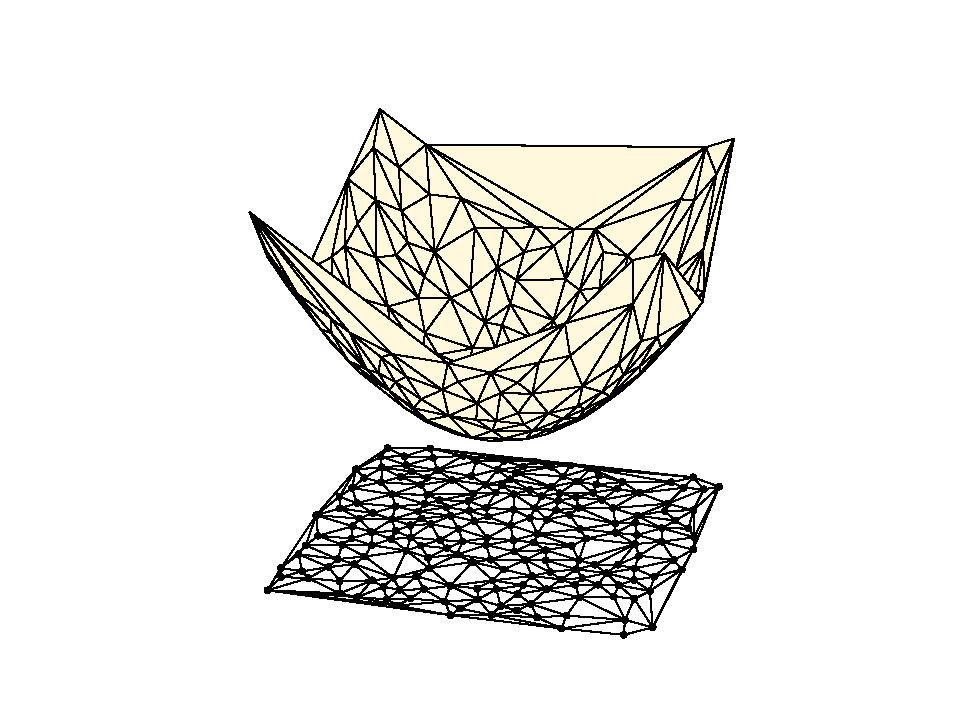
\includegraphics[width=\textwidth]{./appendices/figures/power_3.pdf}
         \caption{}
         \label{appfig:vorconvexhull3}
     \end{subfigure}
     \hspace{1cm}
      \begin{subfigure}[b]{0.4\textwidth}
         \centering
         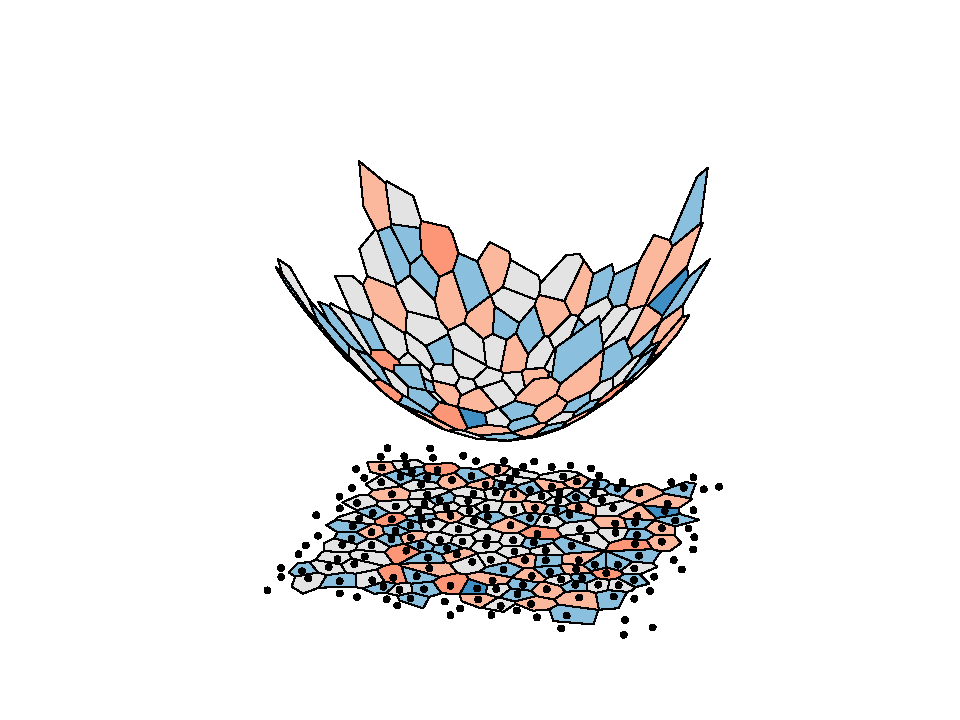
\includegraphics[width=\textwidth]{./appendices/figures/power_4.pdf}
         \caption{}
         \label{appfig:vorconvexhull4}
     \end{subfigure}

	\caption{A point set (panel a) in ${\rm I\!R}^2$ undergoes the lifting transformation, $T$, mapping it onto a paraboloid in ${\rm I\!R}^3$ (panel b). The projection of the lower convex hull back onto the horizontal plane gives the Delaunay triangulation (panel c), from which the Voronoi diagram can be obtained (panel d).}
	\label{appfig:vorconvexhull}
\end{figure}


